\subsection{Explanation of the correlation between Relative turn length and turn changes}
\label{sec:opposite}

Our initial hypothesis \ref{chap:intorduction} was that low relative turn change would lead to a speaker holding the floor, and high relative turn change would lead to a turn change. However, in section \ref {sec:data:summary}, we reported that the relative turn length feature was giving us the opposite effect.
We found that the chance of turn change is higher when the speaker has the floor for shorter than its average turn. Also, the speaker will likely keep the floor when speaking more than the average turn length.

We suspect that the reason that our initial hypothesis proved to be incorrect is due to the nature of the corpus. Figure \ref {fig:turn_dist} shows the actual distribution of turn lengths (in seconds).

\begin{figure}[ht!]
\centering
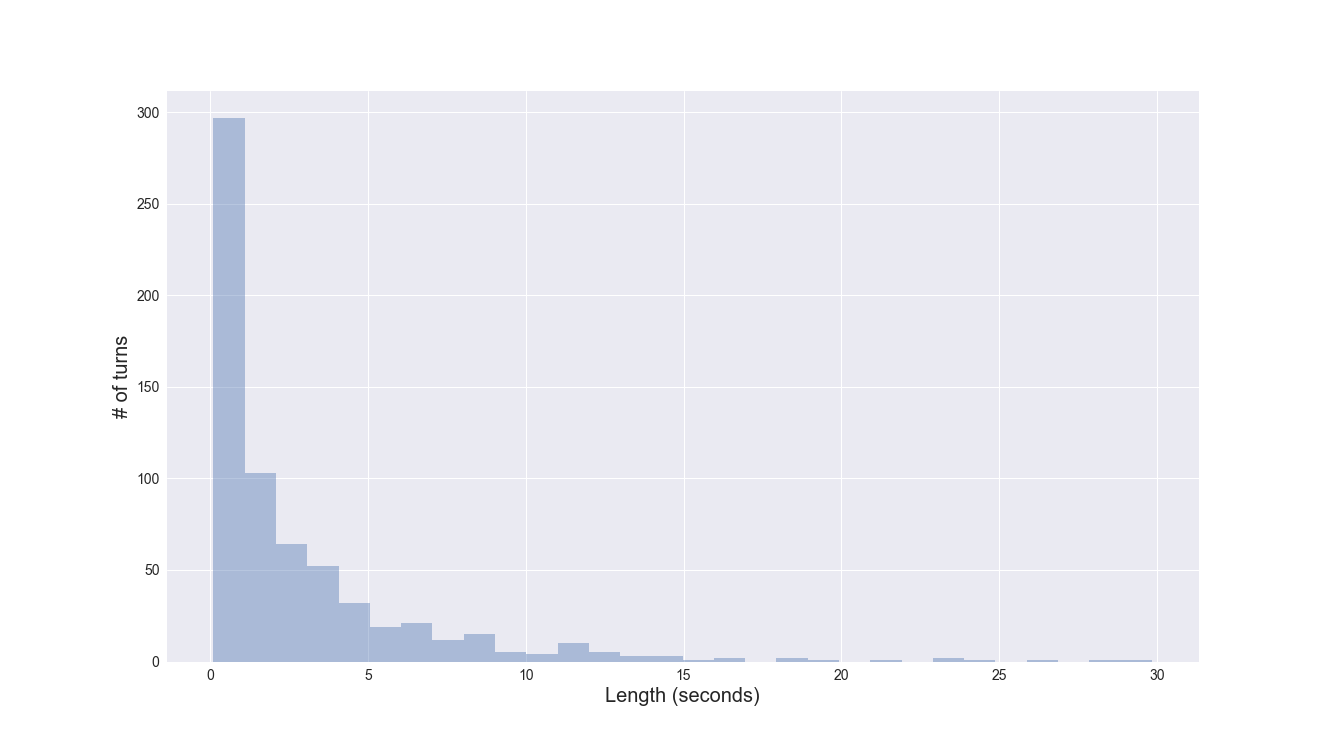
\includegraphics[width=\textwidth]{../scikitlearn/figures/f10.png}\vspace{-1em}
\caption{Distribution of the turn length}
\label{fig:turn_dist}
\end{figure}
%

First we explain why dialog acts with small relative turn length will more likely lead to a turn change. We suspect that the set of short turns is composed of turns with a single dialog act. Moreover, this dialog act is likely to be back channel or an answer, both of which have low relative turn length, see figure \ref{fig:act:turn:rtl}. If we look at figure \ref{fig:act:turnchange}, we can see that the chance of a back channel or a answer causing a turn change is 60-80\%. From both observation we can conclude that a short dialog act with low relative turn length will likely to lead to a turn change.

On the other end, we want to explain why high relative turn length would not lead to a turn change. This can be attributed to the structure of the distribution curve of figure \ref{fig:turn_dist}, which has a long flat tail. Hence if the speaker spoke for high relative turn length, the chance that the current dialog act will lead to a turn change are smaller and smaller and hence the speaker will likely keep the floor.
